
\chapter{Metodi dei Residui Pesati e Applicazioni ai Calcoli di Core}
	
\section{Introduzione al Metodo dei Residui Pesati}
	Il metodo dei residui pesati è una tecnica numerica utilizzata per approssimare la soluzione di problemi differenziali. Consideriamo il seguente problema differenziale alle derivate parziali:
	\[
	L \,\phi(\mathbf{r})\, +\, S(\mathbf{r})\ =\ 0\ \ ,
	\]
	dove \(L\) è un operatore differenziale. Nel caso dell'equazione di diffusione, l'operatore \(L\) assume la forma:
	\[
	L \cdot\ =\ \nabla \cdot D \nabla \cdot - \Sigma_a \cdot\ \ .
	\]
	
	L'obiettivo è trovare una soluzione approssimata \(\tilde{\phi}(\mathbf{r})\) espressa come combinazione lineare di funzioni di prova \(u_j(\mathbf{r})\):
	\[
	\tilde{\phi}(\mathbf{r}) = \sum_{j=1}^N c_j u_j(\mathbf{r}).
	\]
	Le funzioni di prova \(u_j(\mathbf{r})\) devono essere sufficientemente regolari per consentire l'applicazione dell'operatore \(L\) e devono soddisfare le condizioni al contorno del problema.
	
\section{Formulazione del Metodo dei Residui Pesati}
	Sostituendo l'espressione di \(\tilde{\phi}(\mathbf{r})\) nell'equazione originale, otteniamo un residuo \(R(\mathbf{r})\):
	
	\[
	L \tilde{\phi}(\mathbf{r})\, +\, S(\mathbf{r})\ =\ R(\mathbf{r})\ \neq\ 0\ \ .
	\]
	
	Il metodo dei residui pesati richiede che il residuo sia "piccolo" in un senso integrale, imponendo che sia ortogonale ($\left(R(\mathbf r),\, w_i(\mathbf r)\right)$) a un insieme di \(N\) funzioni peso \(w_i(\mathbf{r})\):
	\[
	\int_V\, R(\mathbf{r})\, w_i(\mathbf{r}) \, \mathrm{d}V\ =\ 0, \qquad i\, =\, 1, \dots, N.
	\]
	Questa condizione può essere riscritta come:
	\[
	\int_V \left( L \sum_{j=1}^N c_j u_j(\mathbf{r}) + S(\mathbf{r}) \right) w_i(\mathbf{r}) \, \mathrm{d}V = 0.
	\]
	Sviluppando l'integrale, otteniamo un sistema di \(N\) equazioni nelle \(N\) incognite \(c_j\):
	\[
	\sum_{j=1}^N c_j \int_V L u_j(\mathbf{r}) w_i(\mathbf{r}) \, \mathrm{d}V + \int_V S(\mathbf{r}) w_i(\mathbf{r}) \, \mathrm{d}V = 0.
	\]
	
	In principio, le funzioni di prova $u_j(\mathbf r)$ possono essere funzioni qualsiasi purché rispettino le condizioni al contorno, siano regolari ed è buona cosa che siano anche facili da differenziare ed integrare e che localmente presentino una forma simile alla soluzione esatta. Per questo spesso vengono usati polinomi di basso ordine.
	
%
%
%	
\section{Scelta delle Funzioni Peso}
	La scelta delle funzioni peso \(w_i(\mathbf{r})\) caratterizza il metodo dei residui pesati. Tre scelte classiche sono:
	\begin{itemize}
		\item \textbf{Metodo di Galerkin:} Le funzioni peso coincidono con le funzioni di prova, cioè \(w_i(\mathbf{r}) = u_i(\mathbf{r})\).
		\item \textbf{Metodo dei sottodomini:} Le funzioni peso sono definite come 1 all'interno di un sottodominio e 0 altrimenti.
		\item \textbf{Metodo di collocazione:} Le funzioni peso sono funzioni delta di Dirac, che impongono l'annullamento del residuo in punti specifici del dominio.
	\end{itemize}
	
\subsection{Metodo di Galerkin}
	Nel metodo di Galerkin, le funzioni peso sono scelte tra le funzioni di prova. Ad esempio, in un problema monodimensionale, se il flusso è approssimato da un polinomio di ordine \(N\):
	\[
	\tilde{\phi}(x) = \sum_{i=1}^N c_i u_i(x) = c_0 + c_1 x + c_2 x^2 + \dots + c_N x^N,
	\]
	le funzioni peso possono essere scelte come \(w_i(x) = x^k\) per \(k = 1, \dots, N\).
	
\subsection{Metodo dei Sottodomini}
	Nel metodo dei sottodomini, il dominio di calcolo \(V\) viene suddiviso in sottodomini \(V_m\). Le funzioni peso sono definite come:
	\[
	w_i(\mathbf{r}) = \begin{cases}
		1\ , \quad \text{se } \mathbf{r} \in V_m, \\
		0\ , \quad \text{altrimenti}.
	\end{cases}
	\]
	In ogni sottodominio, si impone che l'integrale del residuo sia nullo:
	\[
	\int_{V_m}\, R(\mathbf{r}) \, \mathrm{d}V\ =\ 0\ \ .
	\]
	\subsubsection{Applicazione del Metodo dei Sottodomini all’Equazione di Diffusione}
	
	Nel caso dell’equazione di diffusione, il metodo dei sottodomini equivale a imporre il bilancio neutronico sul volume \(V_m\):
	\[
	\int_{V_m} R(\mathbf{r}) \, \mathrm{d}V \ =\ 0\ \implies\ \int_{V_m} \left[ \nabla \cdot D \nabla \tilde{\phi} - \Sigma_a \tilde{\phi} + S \right] \, \mathrm{d}V\ =\ 0\ \ .
	\]
	
	Sviluppando l’integrale, si ottiene:
	
	\[
	\int_{S_m} D \nabla \tilde{\phi} \cdot \mathbf{n} \, \mathrm{d}A\, -\, \int_{V_m} \Sigma_a \tilde{\phi} \, \mathrm{d}V \,+\, \int_{V_m} S \, \mathrm{d}V\ =\ 0\ \ .
	\]
	
	Questa equazione può essere interpretata come un bilancio tra le perdite per fuga (leakages), le perdite per assorbimento (absorptions) e la sorgente (source):
	
	\[
	\underbrace{\int_{S_m} \mathbf{J} \cdot \mathbf{n} \, \mathrm{d}A}_{\text{Perdite per fuga}} \,+\, \underbrace{\int_{V_m} \Sigma_a \tilde{\phi} \, \mathrm{d}V}_{\text{Perdite per assorbimento}}\ =\ \underbrace{\int_{V_m} S \, \mathrm{d}V}_{\text{Sorgente}}\ \ .
	\]
	
	Questo è un requisito fondamentale che deve essere soddisfatto da qualsiasi schema numerico.
	
	Tuttavia, il bilancio neutronico deve essere garantito anche sull'intero dominio di calcolo \(V\), imponendo opportune condizioni di continuità della corrente attraverso le interfacce dei sottodomini. Questo assicura che il metodo dei sottodomini non solo approssimi localmente la soluzione, ma preservi anche la coerenza fisica globale del sistema.
	
	
	
\subsection{Metodo di Collocazione}
	Nel metodo di collocazione, le funzioni peso sono funzioni delta di Dirac:
	\[
	w_i(\mathbf{r})\ =\ \delta(\mathbf{r} - \mathbf{r}_i)\ \ .
	\]
	Questo metodo impone che il residuo sia nullo in punti specifici \(\mathbf{r}_i\):
	
	\[\int_V R(\mathbf{r})\, \delta(\mathbf{r} - \mathbf{r}_i) \, \mathrm{d}V\ =\ R(\mathbf{r}_i)\ =\ 0\ \ .\]
	
	Allora il metodo di collocazione è equivalente ad imporre che il residuo sia nullo in una certa posizione $\mathbf r_i$, $\emph{i.e.}$ la soluzione approssimata risolve esattamente l'equazione differenziale in quel punto.
	
	Fissare il residuo a zero in $\mathbf r_i$ non vuol dire che non vi sia errore in quel punto. Per mandare l'errore a zero servirà prendere sempre più funzioni nella sequenza di approssimazione $\tilde\phi$.
	
	
\section{Applicazione al Calcolo del Core del Reattore}
	Il core di un reattore nucleare è caratterizzato da una geometria complessa, che può essere semplificata attraverso un processo di omogeneizzazione. Questo processo trasforma la geometria reale in una serie di celle omogeneizzate, che possono essere trattate come nodi in una griglia grossolana. Ogni nodo rappresenta una sezione assiale di un'assemblaggio, e il flusso neutronico viene approssimato all'interno di ogni nodo utilizzando polinomi.
	
	\begin{figure}[H]
		\centering
		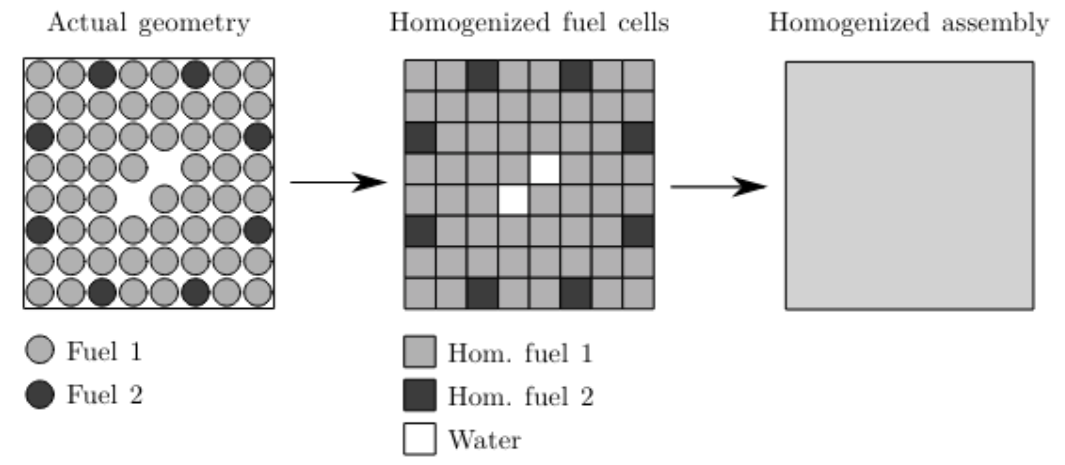
\includegraphics[width=11cm]{img/coarse-mesh1.png}
		\label{fig:}
		\caption{}
	\end{figure}
	
\section{Applicazione del Metodo dei Sottodomini}

\subsection{Formulazione del Bilancio Neutronico}
Applicando il metodo dei sottodomini, si impone che l'integrale del residuo su ogni volume \(V_{ijl}\) sia nullo:
\[
\int_{V_{ijl}} \left[ \nabla \cdot D \nabla \phi - \Sigma_a \phi + \frac{\nu}{k} \Sigma_f \phi \right] \, \mathrm{d}V = 0.
\]
Questa condizione equivale a imporre il bilancio neutronico su ogni sottodominio \(V_{ijl}\). Scomponendo l'integrale, si ottiene:
\[
\int_{V_{ijl}} \nabla \cdot D \nabla \phi \, \mathrm{d}V = \int_{\partial V_{ijl}} D \nabla \phi \cdot \mathbf{n} \, \mathrm{d}A.
\]
Sviluppando ulteriormente, si arriva a espressioni che coinvolgono le derivate del flusso alle interfacce del nodo, ad esempio:
\[
\int_{V_{ijl}} \nabla \cdot D \nabla \phi \, \mathrm{d}V = D_{ijl} \left[ \frac{\partial \phi}{\partial x} \bigg|_{x_{i+\frac{1}{2}}} - \frac{\partial \phi}{\partial x} \bigg|_{x_{i-\frac{1}{2}}} \right] h_{y_j} h_{z_l} + \dots
\]
dove \(\frac{\partial \phi}{\partial x}\) è espresso in termini dei coefficienti \(a_{x,ijl}\) e \(b_{x,ijl}\):
\[
\frac{\partial \phi}{\partial x} = \phi_{ijl} \left[ \frac{a_{x,ijl}}{h_{x_i}} + \frac{2(x - x_i)}{h_{x_i}^2} b_{x,ijl} \right].
\]
Sostituendo e semplificando, si ottiene:
\[
\int_{V_{ijl}} \nabla \cdot D \nabla \phi \, \mathrm{d}V = \phi_{ijl} D_{ijl} V_{ijl} \frac{2 b_{x,ijl}}{h_{x_i}^2} + \dots
\]
dove \(V_{ijl} = h_{x_i} h_{y_j} h_{z_l}\).

\subsection{Integrazione del Termine di Assorbimento e Sorgente}
Il termine di assorbimento e sorgente viene integrato come segue:
\[
\int_{V_{ijl}} \left( \frac{\nu}{k} \Sigma_f - \Sigma_a \right) \phi \, \mathrm{d}V = \left( \frac{\nu}{k} \Sigma_f - \Sigma_a \right)_{ijl} \int_{V_{ijl}} \phi \, \mathrm{d}V.
\]
Utilizzando la trasformazione di coordinate \(\mathrm{d}V = V_{ijl} \, \mathrm{d}\xi \, \mathrm{d}\eta \, \mathrm{d}\zeta\), l'integrale del flusso diventa:
\[
\int_{V_{ijl}} \phi \, \mathrm{d}V = \phi_{ijl} V_{ijl} \left(1 + \frac{b_{x,ijl} + b_{y,ijl} + b_{z,ijl}}{12}\right).
\]

\subsection{Equazione Discretizzata}
Combinando i risultati precedenti, si ottiene l'equazione discretizzata:
\[
2 D_{ijl} \left( \frac{b_{x,ijl}}{h_{x_i}^2} + \frac{b_{y,ijl}}{h_{y_i}^2} + \frac{b_{z,ijl}}{h_{z_l}^2} \right) \phi_{ijl} + \left( \frac{\nu}{k} \Sigma_f - \Sigma_a \right)_{ijl} \left( 1 + \frac{b_{x,ijl} + b_{y,ijl} + b_{z,ijl}}{12} \right) \phi_{ijl} = 0.
\]
I coefficienti \(b\) sono espressi in termini dei flussi alle interfacce:
\[
b_{x,ijl} = 2 \frac{\phi_{i+\frac{1}{2},jl} - 2\phi_{ijl} + \phi_{i-\frac{1}{2},jl}}{\phi_{ijl}}, \quad b_{y,ijl} = 2 \frac{\phi_{i,j+\frac{1}{2},l} - 2\phi_{ijl} + \phi_{i,j-\frac{1}{2},l}}{\phi_{ijl}}, \quad b_{z,ijl} = 2 \frac{\phi_{ij,l+\frac{1}{2}} - 2\phi_{ijl} + \phi_{ij,l-\frac{1}{2}}}{\phi_{ijl}}.
\]

\subsection{Condizioni di Continuità della Corrente}
Per garantire il bilancio neutronico globale, è necessario imporre la continuità della corrente alle interfacce dei nodi. Ad esempio, per l'interfaccia a \(x_{i+\frac{1}{2}}\):
\[
- D_{ijl} \frac{\partial \phi}{\partial x} \bigg|_{x_{i+\frac{1}{2}}} = - D_{i+1,jl} \frac{\partial \phi}{\partial x} \bigg|_{x_{i+1-\frac{1}{2}}}.
\]
Sostituendo le espressioni per \(\frac{\partial \phi}{\partial x}\) e semplificando, si ottiene una relazione per il flusso all'interfaccia:
\[
\phi_{i+\frac{1}{2},jl} = \frac{\left(4 - \frac{\phi_{i-\frac{1}{2},jl}}{\phi_{ijl}}\right)}{3 \left(1 + \frac{D_{i+1,jl}}{D_{ijl}} \frac{h_{x_i}}{h_{x_{i+1}}}\right)} \phi_{ijl} + \frac{\left(4 - \frac{\phi_{i+\frac{3}{2},jl}}{\phi_{i+1,jl}}\right)}{3 \left(1 + \frac{D_{ijl}}{D_{i+1,jl}} \frac{h_{x_{i+1}}}{h_{x_i}}\right)} \phi_{i+1,jl}.
\]
Questa relazione può essere scritta in forma compatta come:
\[
\phi_{i+\frac{1}{2},jl}^{(n)} = \alpha_{(i,i+1),jl}^{(n)} \phi_{ijl}^{(n)} + \beta_{(i,i+1),jl}^{(n)} \phi_{i+1,jl}^{(n)}.
\]

\subsection{Equazione a 7 Punti}
Sostituendo le espressioni per i flussi alle interfacce nell'equazione discretizzata, si ottiene un'equazione a 7 punti:
\[
O_{ijl} \phi_{ijl} + W_{ijl} \phi_{i-1,jl} + E_{ijl} \phi_{i+1,jl} + S_{ijl} \phi_{i,j-1,l} + N_{ijl} \phi_{i,j+1,l} + D_{ijl} \phi_{ij,l-1} + U_{ijl} \phi_{ij,l+1} = 0.
\]
I coefficienti \(O_{ijl}, W_{ijl}, \dots\) sono più complessi rispetto al caso delle differenze finite, ma permettono di ottenere una maggiore accuratezza con un numero minore di nodi.

\section{Metodo CUBBOX}

\subsection{Approssimazione del Flusso con Polinomi di Terzo Ordine}
Nel metodo CUBBOX, il flusso in ogni nodo è approssimato da un polinomio di terzo ordine:
\[
\phi(x, y, z) = \phi(\xi, \eta, \zeta) = \phi_{ijl} \left(1 + a_{x,ijl} \xi + b_{x,ijl} \xi^2 + c_{x,ijl} \xi \left(\xi^2 - \frac{1}{4}\right) + \dots \right).
\]
Il termine aggiuntivo \(c_{x,ijl} \xi \left(\xi^2 - \frac{1}{4}\right)\) è nullo alle interfacce del nodo e non contribuisce all'integrale del residuo, quindi l'equazione discretizzata rimane valida.

\subsection{Determinazione dei Coefficienti \(c_x, c_y, c_z\)}
I coefficienti \(c_x, c_y, c_z\) sono determinati applicando nuovamente il metodo dei residui pesati con pesi di Galerkin:
\[
w_1 = \xi \left(\xi^2 - \frac{1}{4}\right), \quad w_2 = \eta \left(\eta^2 - \frac{1}{4}\right), \quad w_3 = \zeta \left(\zeta^2 - \frac{1}{4}\right).
\]
Si ottengono così tre equazioni aggiuntive:
\[
-6 \frac{D_{ijl}}{h_{x_i}^2} c_x - \left( \frac{\nu \Sigma_{f,ijl}}{k} - \Sigma_{a,ijl} \right) a_x + \frac{1}{7} \left( \frac{\nu \Sigma_{f,ijl}}{k} - \Sigma_{a,ijl} \right) c_x = 0,
\]
e analogamente per \(c_y\) e \(c_z\). Imponendo le condizioni di continuità della corrente alle interfacce, si ottengono relazioni simili a quelle del metodo QUABOX, ma con coefficienti \(\alpha\) e \(\beta\) ancora più complessi.

\section{Conclusione}
I metodi a maglia grossolana (coarse mesh) permettono di ottenere una distribuzione del flusso più accurata rispetto alle tecniche a volumi finiti, pur richiedendo un costo computazionale maggiore per nodo. Tuttavia, è possibile utilizzare un numero minore di nodi per ottenere la stessa accuratezza, riducendo così il tempo di calcolo complessivo. Le equazioni si riducono a schemi a 3, 5 o 7 punti a seconda della dimensionalità del problema.